\documentclass[UTF8]{ctexart}
% 基本设置和必要宏包
\usepackage{geometry}
\geometry{a4paper,scale=0.8}

% 数学相关宏包
\usepackage{amsmath}
\usepackage{amssymb}
\usepackage{amsfonts}

\usepackage{mathtools}
\usepackage{amsbsy}
\usepackage{amstext}
\usepackage{wasysym}
\usepackage{stmaryrd}
\usepackage{mathrsfs}

% 图形和颜色
%\usepackage{xcolor}
\usepackage{graphicx}
\usepackage{subcaption}
\usepackage{caption}
\usepackage{float}


% 其他功能性宏包
\usepackage{titlesec}
\usepackage{fancyhdr}
\usepackage{setspace}
\usepackage{cite}
\usepackage{appendix}
\usepackage{listings}
\usepackage{pdfpages}
\usepackage{enumitem}
\usepackage{tabu}
\usepackage{threeparttable}
\usepackage{booktabs}
\usepackage{abstract}
\usepackage{multirow}


\usepackage{diagbox} 


% 允许公式跨页
\allowdisplaybreaks[4]



\newcommand{\sihaoheiti}{\fontsize{14pt}\selectfont\heiti}
% 设置全局字体
%\setCJKmainfont{SimSun} % 设置正文为宋体
%\setCJKsansfont{SimHei} % 设置无衬线字体为黑体

% 论文题目设置为三号黑体字,并居中
\newcommand{\threelargebf}{\fontsize{16pt}{19.2pt}\selectfont\heiti\centering}

% 一级标题设置为四号黑体字,并居中
\titleformat{\section}{\centering\fontsize{14pt}{16pt}\bfseries\heiti}{\thesection}{1em}{}

% 二级标题设置为小四号黑体字,左对齐
\titleformat{\subsection}{\fontsize{12pt}{14.4pt}\bfseries\heiti}{\thesubsection}{1em}{\raggedright}

% 三级标题设置为小四号黑体字,左对齐
\titleformat{\subsubsection}{\fontsize{12pt}{14.4pt}\bfseries\heiti}{\thesubsubsection}{1em}{\raggedright}

% 正文字体设置为小四号宋体字,并使用单倍行距
\renewcommand{\normalsize}{\fontsize{12pt}{14.4pt}\selectfont}




%\linespread{5.0}%修改行距
% 图片文件夹
\graphicspath{{img/}{img1/}}


\let\itemize\compactitem
\let\enditemize\endcompactitem
% 设置页面布局
\geometry{a4paper, left=2.5cm, right=2.5cm, top=3cm, bottom=3cm}
\setstretch{1.2}

\renewcommand{\arraystretch}{1.5}
\newcommand{\thickhline}{\noalign{\hrule height 1.2pt}} % 设置粗线的宽度
\newcommand{\thinhline}{\noalign{\hrule height 0.8pt}} % 设置细线的宽度

%%%% ===== 定理环境
\usepackage[amsmath,thref,thmmarks,hyperref]{ntheorem} % 定理宏包
%\theorempreskipamount1em % spacing before the environment
%\theorempostskipamount0em  % spacing after the environment
%\theoremstyle{plain}
%\theoremheaderfont{\normalfont\heiti}
%\theorembodyfont{\normalfont\kaishu}
%\theoremindent0em
%\theoremseparator{\hspace{0.2em}}
%\theoremnumbering{arabic}

\newtheorem{property}{性质}[section]
\newtheorem{definition}{定义}[section]
\newtheorem{lemma}{引理}[section]
\newtheorem{remark}{注记}[section]
\newtheorem{corollary}{推论}[section]
\newtheorem{example}{例}[section] 
\newtheorem{problem}{{问题}}

 \renewcommand{\abstractnamefont}{\normalfont\bfseries}  % 摘要标题字体:正常字体,粗体
\renewcommand{\abstracttextfont}{\normalfont\normalsize}     % 摘要内容字体:正常字体,小四号

% 设置页眉页脚
\pagestyle{fancy}
\fancyhf{}
\fancyfoot[C]{\thepage}
\renewcommand{\headrulewidth}{0pt}

% 设置标题格式
\titleformat{\section}{\centering\heiti\large}{\thesection}{1em}{}
\titleformat{\subsection}{\raggedright\heiti\normalsize}{\thesubsection}{1em}{}
\titleformat{\subsubsection}{\raggedright\heiti\normalsize}{\thesubsubsection}{1em}{}

% 设置摘要环境
%\newenvironment{myabstract}{
%	\begin{center}
%	\bfseries\zihao{-3} 摘要
%	\end{center}
%	\vspace{-0.5em} % 调整摘要与论文题目的距离
%	\normalsize
%}{
%}
% 设置附录环境
\renewcommand{\appendixname}{附录}
\renewcommand{\appendixpagename}{附录}

% 设置代码环境
\lstset{
	basicstyle=\small\ttfamily,
	keywordstyle=\color{blue},
	commentstyle=\color{green!70!black},
	stringstyle=\color{red},
	breaklines=true,
	numbers=left,
	numberstyle=\tiny,
	frame=tb,
	language=Python
}
\newcommand{\bbA}{\mathbb{A}}
\newcommand{\bbB}{\mathbb{B}}
\newcommand{\bbC}{\mathbb{C}}
\newcommand{\bbD}{\mathbb{D}}
\newcommand{\bbE}{\mathbb{E}}
\newcommand{\bbF}{\mathbb{F}}
\newcommand{\bbG}{\mathbb{G}}
\newcommand{\bbH}{\mathbb{H}}
\newcommand{\bbI}{\mathbb{I}}
\newcommand{\bbJ}{\mathbb{J}}
\newcommand{\bbK}{\mathbb{K}}
\newcommand{\bbL}{\mathbb{L}}
\newcommand{\bbM}{\mathbb{M}}
\newcommand{\bbN}{\mathbb{N}}
\newcommand{\bbO}{\mathbb{O}}
\newcommand{\bbP}{\mathbb{P}}
\newcommand{\bbQ}{\mathbb{Q}}
\newcommand{\bbR}{\mathbb{R}}
\newcommand{\bbS}{\mathbb{S}}
\newcommand{\bbT}{\mathbb{T}}
\newcommand{\bbU}{\mathbb{U}}
\newcommand{\bbV}{\mathbb{V}}
\newcommand{\bbW}{\mathbb{W}}
\newcommand{\bbX}{\mathbb{X}}
\newcommand{\bbY}{\mathbb{Y}}
\newcommand{\bbZ}{\mathbb{Z}}

\title{}
\author{}
\date{}

\begin{document}


\begin{titlepage}		
		
\includepdf[pages=-]{封面.pdf}
\end{titlepage}

\section{实验内容}

\begin{enumerate}
    \item 信号发生器输出端接示波器通道$CH1$,选择 Highz,按下 wareform 键选择波形,按下 FREQ/Rate键输入一个不太小的频率,再按 AMPL 键选择 VPP 电压,最后按下 Output 键输出
    一个稳定的信号。观察波形并迅速调出稳定的波形,将信号发生器频率调节为$500\ Hz$,调节示波器出现两个完整的正弦波形,记录其波形;同时调节信号发生器频率分别为$250\ Hz$、$1.5k \ Hz $并记录其波形
    \item 信号发生器输出端接示波器通道$CH2$,校准$X$轴单位格的时间值,分别调节频率至$50 \ Hz$、$150 \ Hz$、$750 \ Hz$、$5k \ Hz$、$50k \ Hz$调整示波器是屏上波形稳定后读出时间
    \item 在上述基础上另一个输出端连接到$CH1$,同时将时间选择至$X-Y$模式调节信号发生器信号的频率$f_x :f_y$比值为$1:1$、$2:1$、$3:1$、$1:4$、$2:3$、$3:4$、$3:5$,记录李萨如法测得的频率$f_x$、$f_y$和图像
    \item 校准$CH2$输入的灵敏度,用示波器直接测量信号发生器电压输出为$2\ V$、$5 \ V$、$7 \ V$、$10 \ V$时的峰值和有效值
\end{enumerate}


\section{原始数据}
\begin{table}[H]
    \centering
    \caption{接$CH2$改变信号频率测量时间}
    \begin{tabular}{|c|c|c|c|c|c|}
    \hline
         频率$/Hz$ & 50 & 150 & 750 & 5k & 50k \\
    \hline
         时间 & $21 \ ms$  & $7.1 \ ms$ & $ 1.4 \ ms$ & $210 \ \mu s$ & $20 \ \mu s$ \\
    \hline
    \end{tabular}
\end{table}
记录得垂直衰减选择旋钮对应为$2.00 \ V$
\begin{table}[H]
    \centering
    \caption{李萨如法测频率}
    \begin{tabular}{|c|c|c|c|c|c|c|c|}
    \hline
         $f_x :f_y$ & $1:1$ & $2:1$ & $3:1$ & $1:4$ & $2:3$ & $3:4$ & $3:5$ \\
    \hline
          $f_x/ Hz$  & $500$  & $1000$ & $1500$ & $250$  & $1.0k$ & $1.5k$ & $1.5k$ \\
    \hline
           $f_y/ Hz$  & $500$  & $500$ & $500$ & $1.0k$  & $1.5k$ & $2.0k$ & $2.5k$ \\
    \hline 
    \end{tabular}
\end{table}

\begin{table}[H]
    \centering
    \caption{用示波器测电压}
    \begin{tabular}{|c|c|c|c|c|}
    \hline
        信号发生器电压输出值$/V$ & 2 & 5  & 7 & 10   \\
    \hline
        峰值$/V$ & $1.2$ & $2.7$ & $3.7$ & $5.5$ \\
    \hline
        有效值$/V$ & $\frac{1.2}{\sqrt{2}}$ & $\frac{2.7}{\sqrt{2}}$ & $\frac{3.7}{\sqrt{2}}$ & $\frac{5.5}{\sqrt{2}}$ \\
    \hline
    \end{tabular}
\end{table}

\section{数据处理与分析}
\subsection{观察与调出稳定波形}
键钮的功能与方法
\begin{enumerate}
    \item 触发源  \Large{\textcircled{\small{23}}}\normalsize :内部触发源信号以及外部$EXT\  TRIG.IN$输入信号选择器,用于改变接入源
    \item 触发电平 \Large{\textcircled{\small{28}}}\normalsize:同步波形,并设定该波形的起始点,同时电平触发同步后使信号同步稳定;\Large{\textcircled{\small{26}}}\normalsize:选择信号通过正向或负向触发
    \item 扫描时间旋钮 \Large{\textcircled{\small{29}}}\normalsize:扫描时间选择旋钮,用于调整扫描周期以获得稳定波形;\Large{\textcircled{\small{30}}}\normalsize:扫描时间可变控制旋钮,用于校准扫描数值
    \item 垂直衰减选择旋钮 \large{\textcircled{\small{7}}}\normalsize:选择$CH1$和$CH2$输入信号的衰减幅度,旋钮选择电压量程;和灵敏度微调控制 
 \large{\textcircled{\small{9}}}\normalsize:电位器可微调电压量程,顺时针旋到底部校正
\end{enumerate}

图形如下
\vspace{13cm}
% 老师会发坐标纸,把课上调出的波形管绘制在上面即可


原因:改变输入信号的频率时相应周期也会发生改变,从而使获得的图像个数不同;





\newpage
\subsection{测量信号频率}
原始数据中测得时间如下
\begin{table}[H]
    \centering
    \caption*{接$CH2$改变信号频率测量时间}
    \begin{tabular}{|c|c|c|c|c|c|}
    \hline
         频率$/Hz$ & 50 & 150 & 750 & 5k & 50k \\
    \hline
         时间 & $21 \ ms$  & $7.1 \ ms$ & $ 1.4 \ ms$ & $210 \ \mu s$ & $20 \ \mu s$ \\
    \hline
    \end{tabular}
\end{table}
此时根据公式$f = \frac{1}{T} $可得
\begin{table}[H]
    \centering
    \caption*{接$CH2$改变信号频率测量时间}
    \begin{tabular}{|c|c|c|c|c|c|}
    \hline
         时间 & $21 \ ms$  & $7.1 \ ms$ & $ 1.4 \ ms$ & $210 \ \mu s$ & $20 \ \mu s$ \\
    \hline
        频率$/Hz$ & 47.6  & 140.8 &  714.3 & 4761.9 & 50000 \\
    \hline
    \end{tabular}
\end{table}



\begin{figure}[H]
	\centering
	\begin{minipage}{0.49\linewidth}
		\centering
		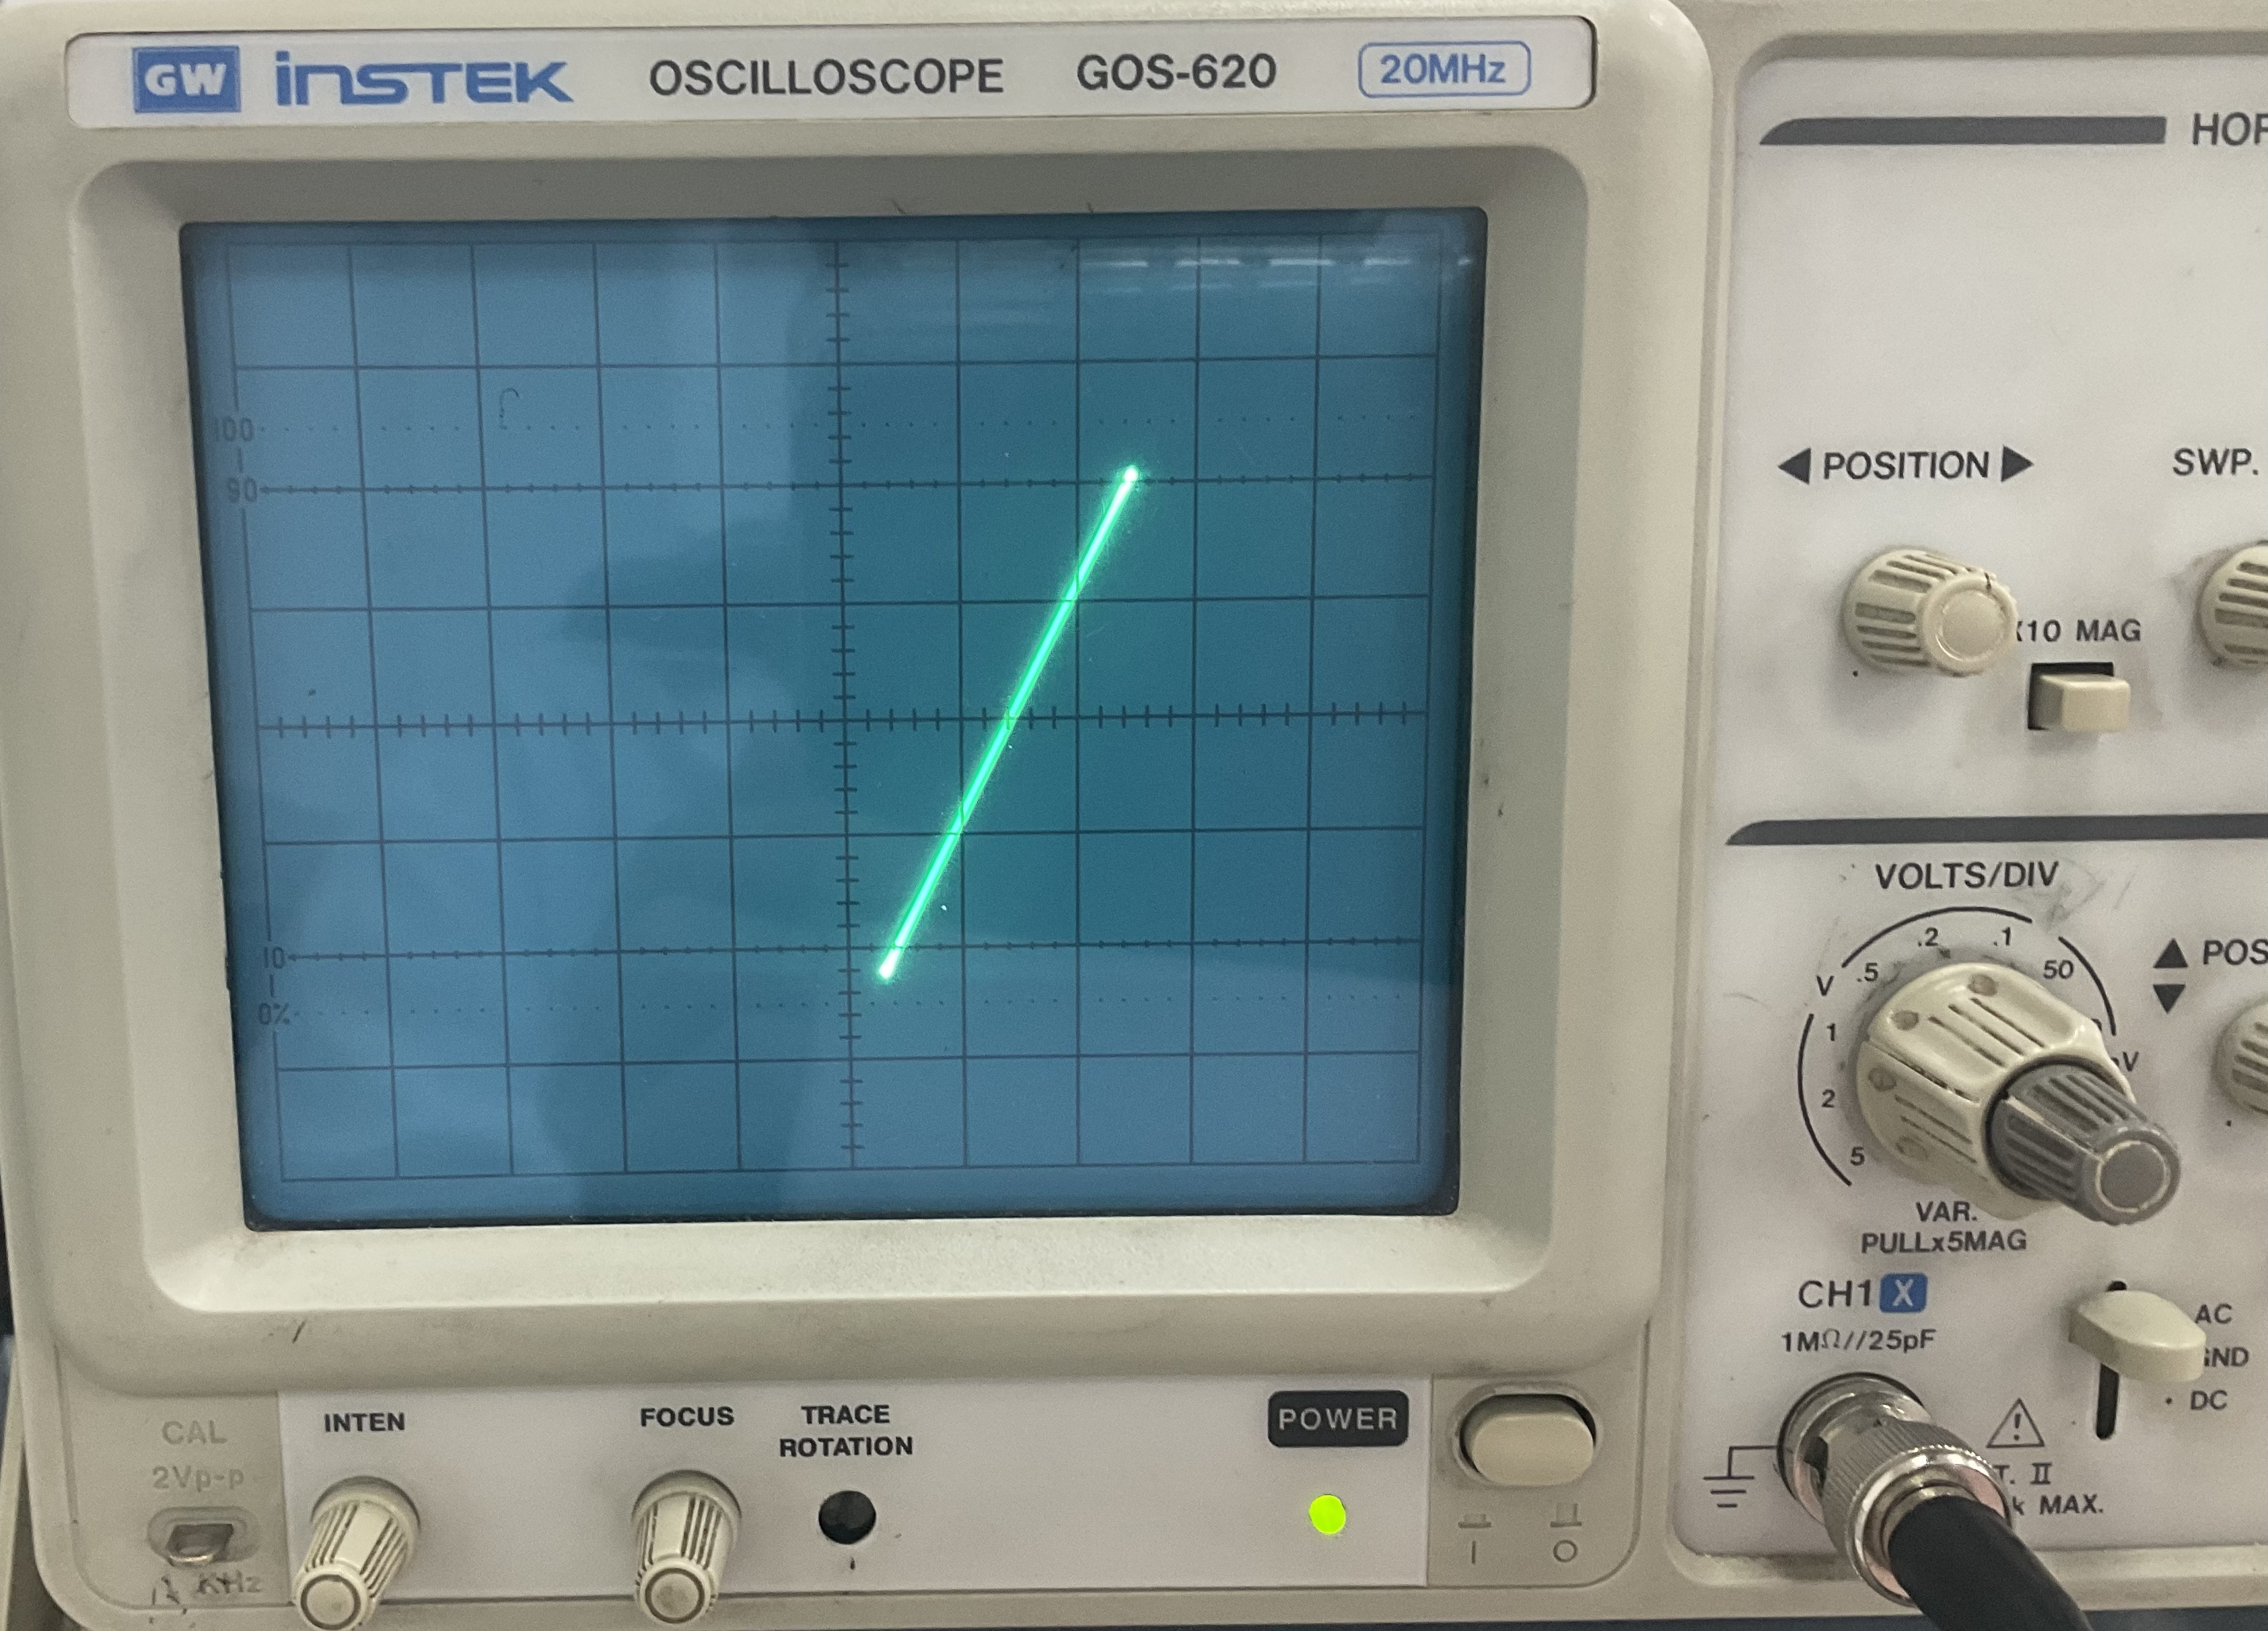
\includegraphics[width=0.9\linewidth]{img1/1比1.jpg}
		\caption*{$f_x:f_y=1:1$}
	\end{minipage}
	\begin{minipage}{0.49\linewidth}
		\centering
		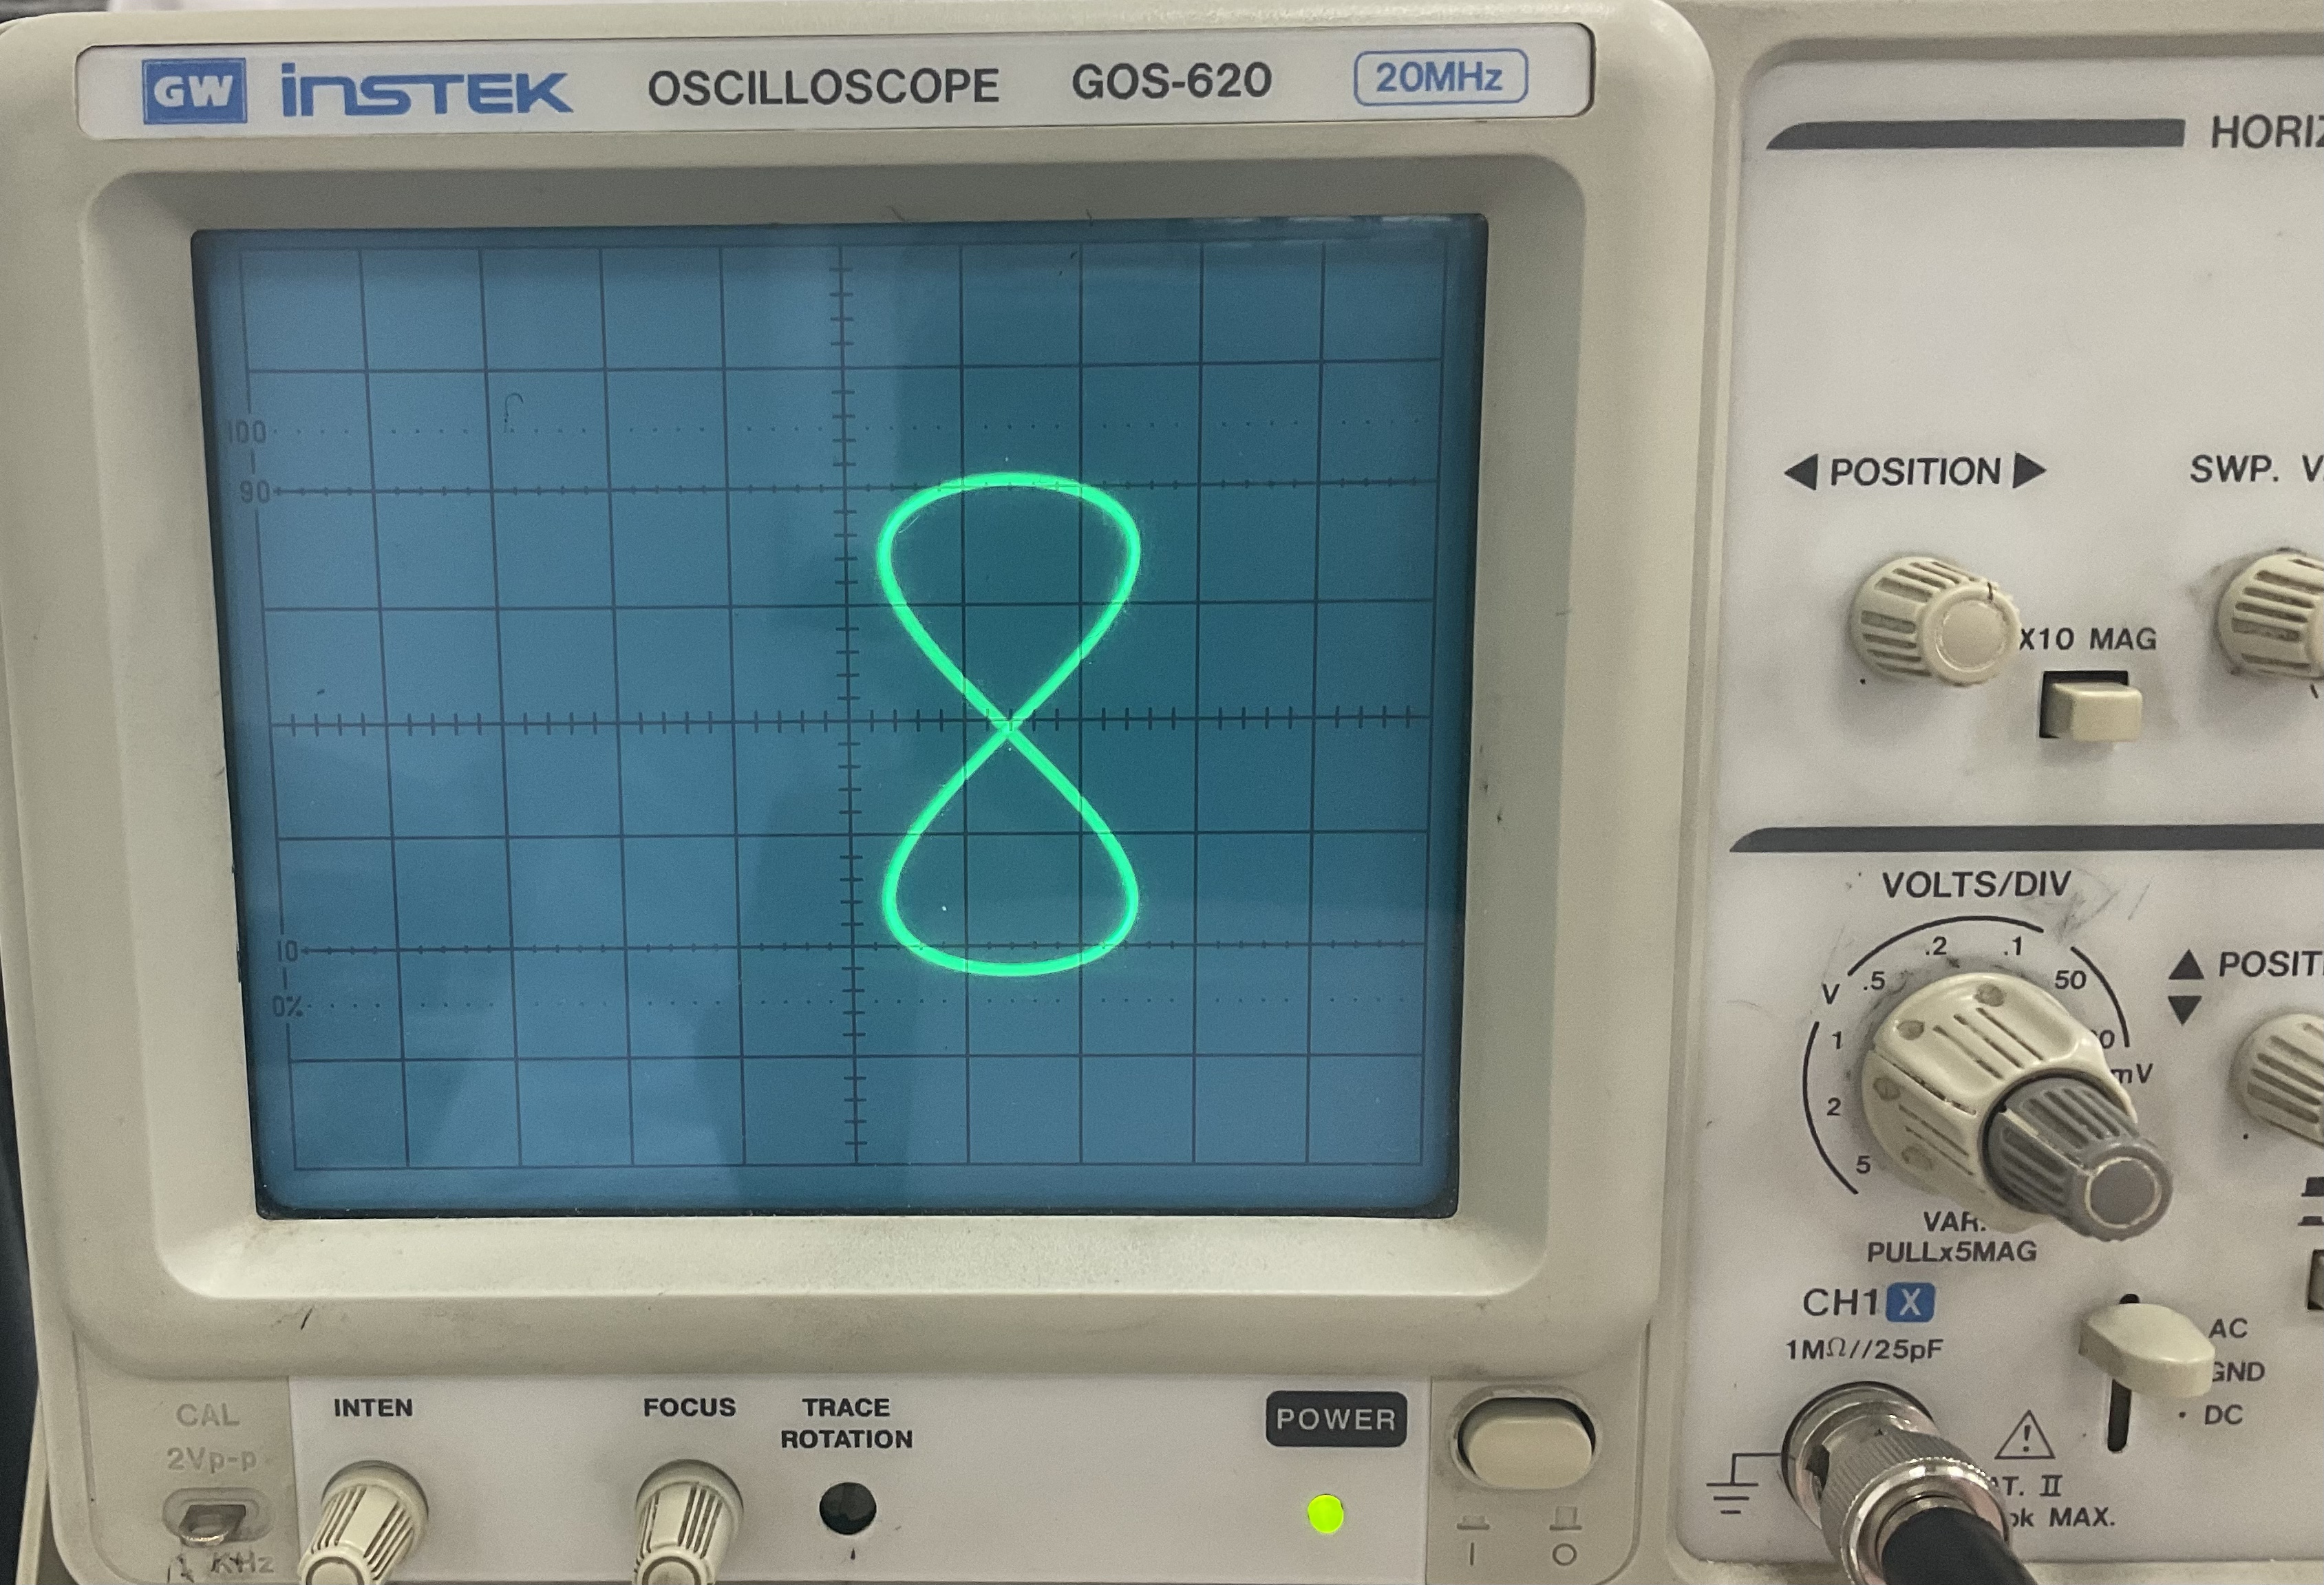
\includegraphics[width=0.9\linewidth]{img1/2比1.jpg}
		\caption*{$f_x:f_y=2:1$}
	\end{minipage}
	%\qquad
	%让图片换行,
	
	\begin{minipage}{0.49\linewidth}
		\centering
		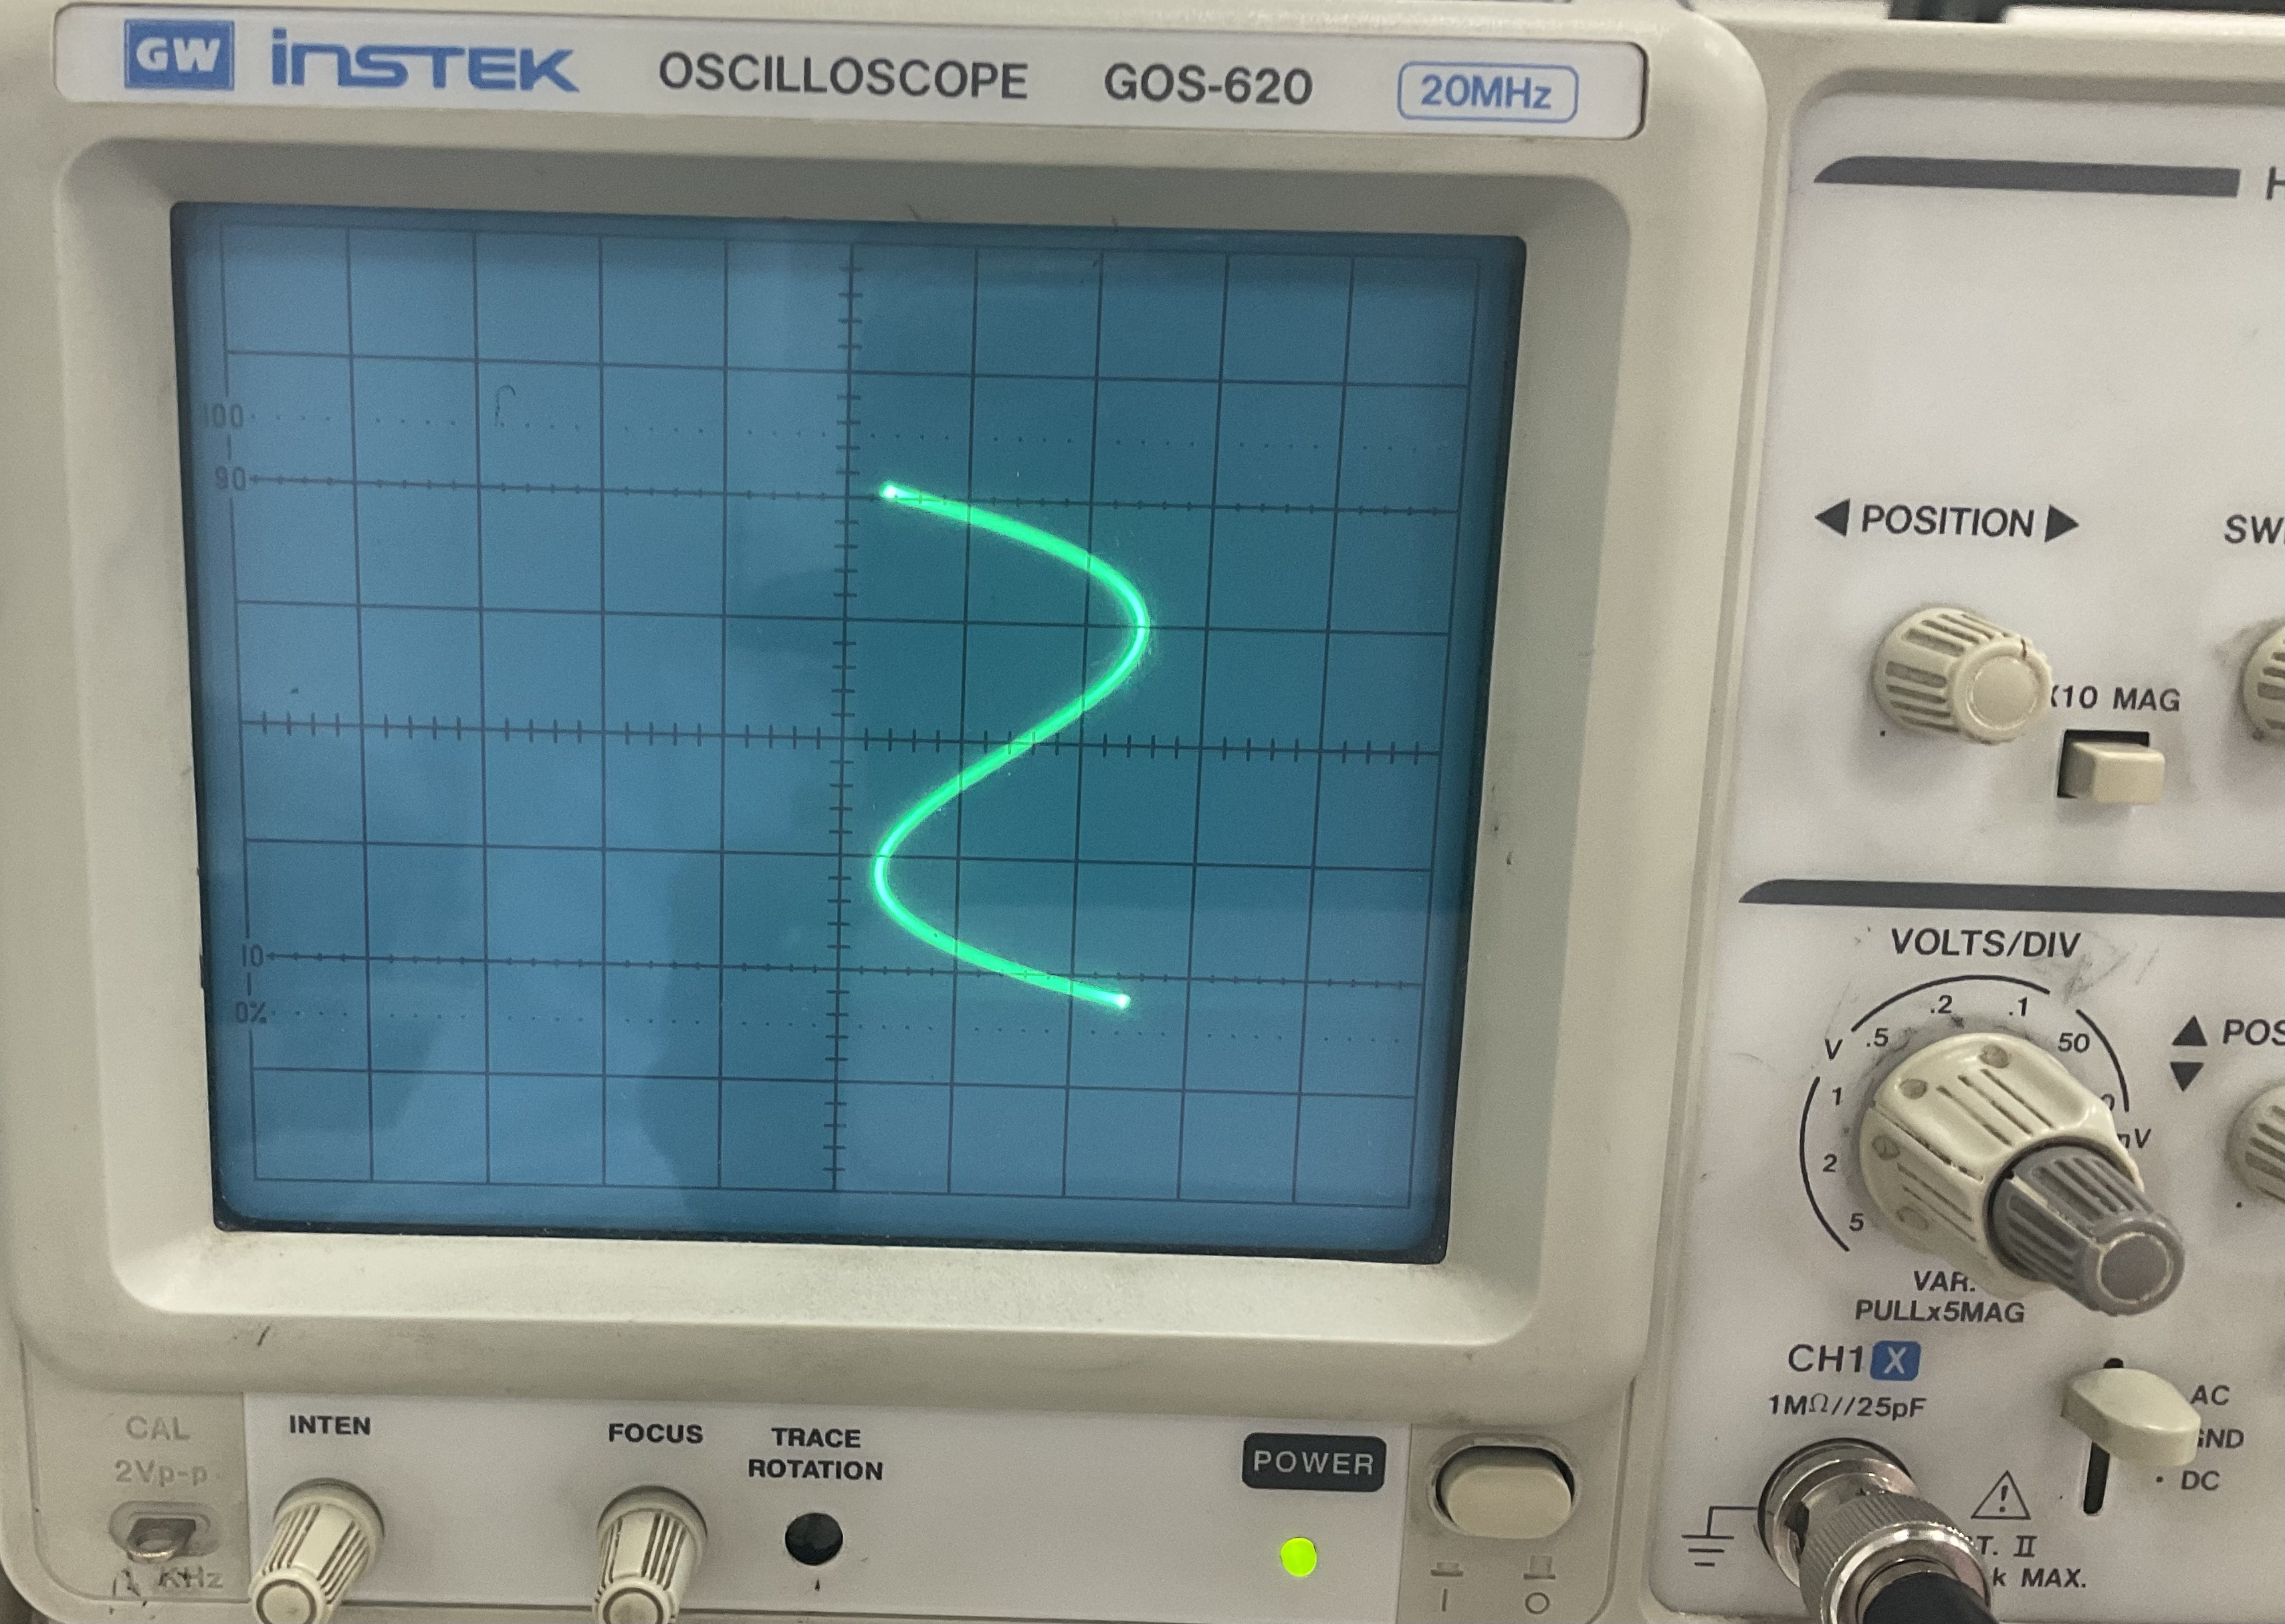
\includegraphics[width=0.9\linewidth]{img1/3比1.jpg}
		\caption*{$f_x:f_y=3:1$}
	\end{minipage}
	\begin{minipage}{0.49\linewidth}
		\centering
		\includegraphics[width=0.9\linewidth]{img1/1比4.jpg}
		\caption*{$f_x:f_y=1:4$}
	\end{minipage}
\end{figure}



\begin{figure}[H]
	\centering
	\begin{minipage}{0.49\linewidth}
		\centering
		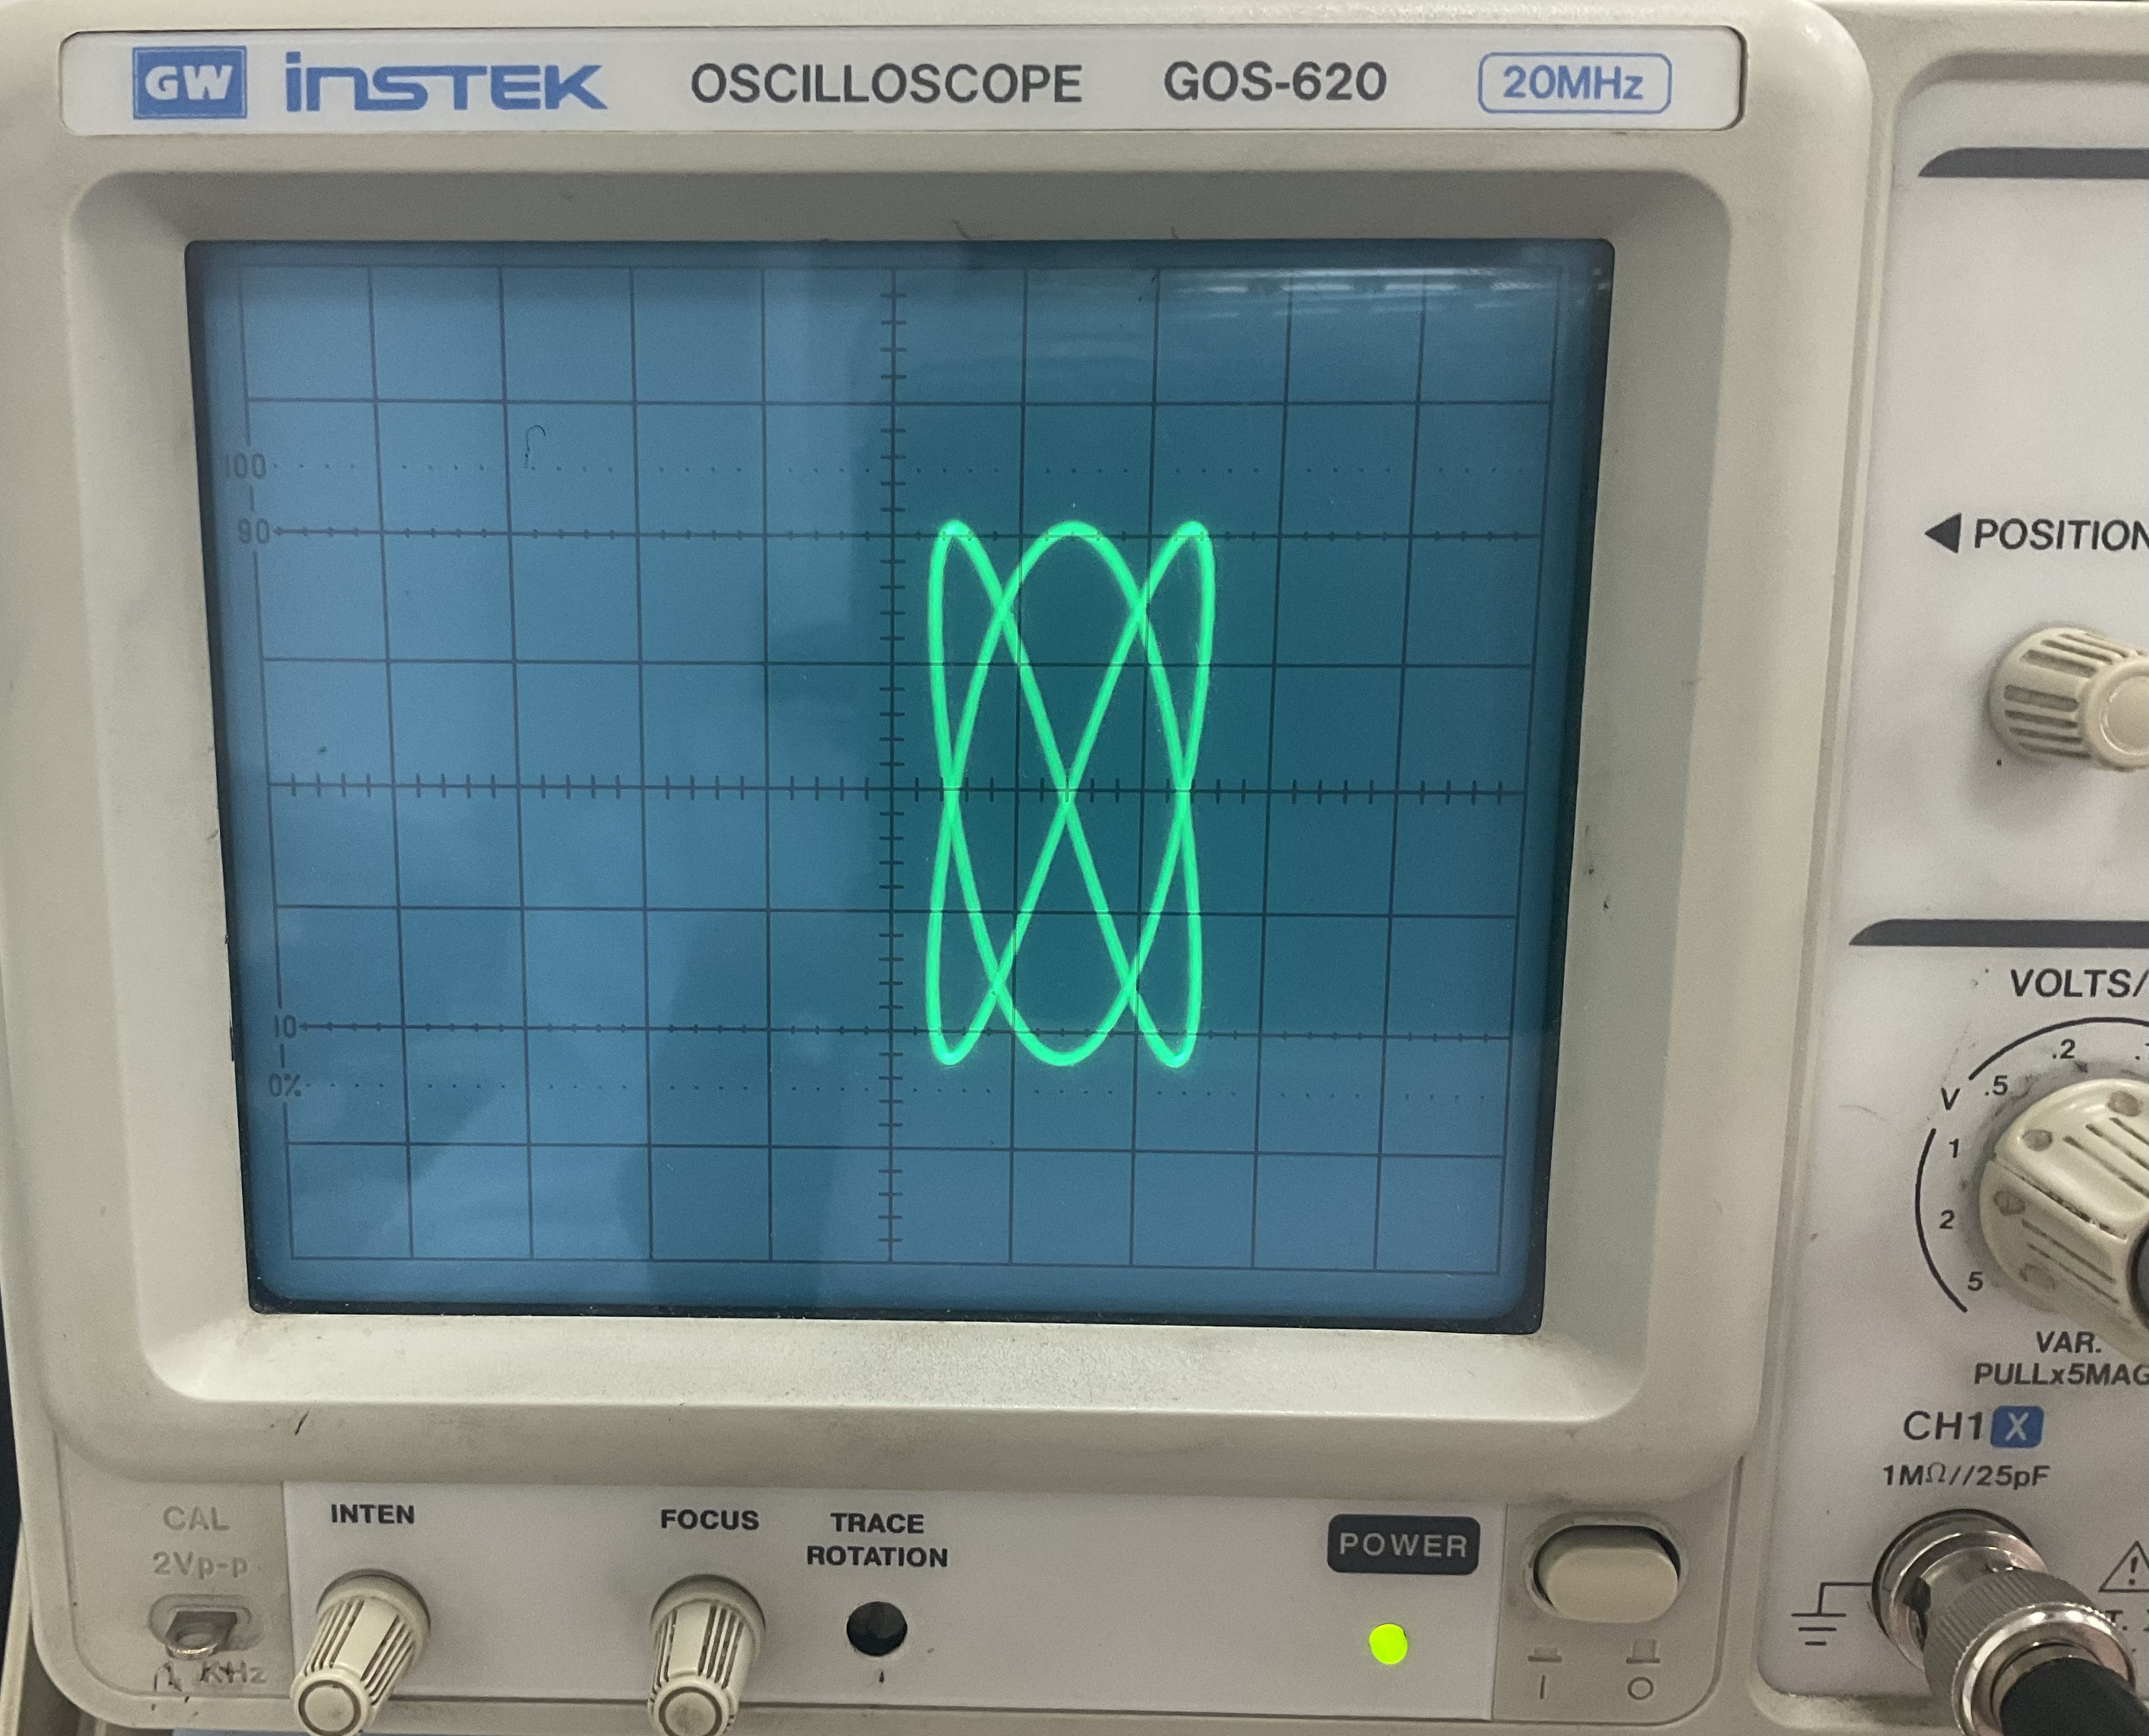
\includegraphics[width=0.9\linewidth]{img1/2比3.jpg}
		\caption*{$f_x:f_y=2:3$}
	\end{minipage}
	\begin{minipage}{0.49\linewidth}
		\centering
		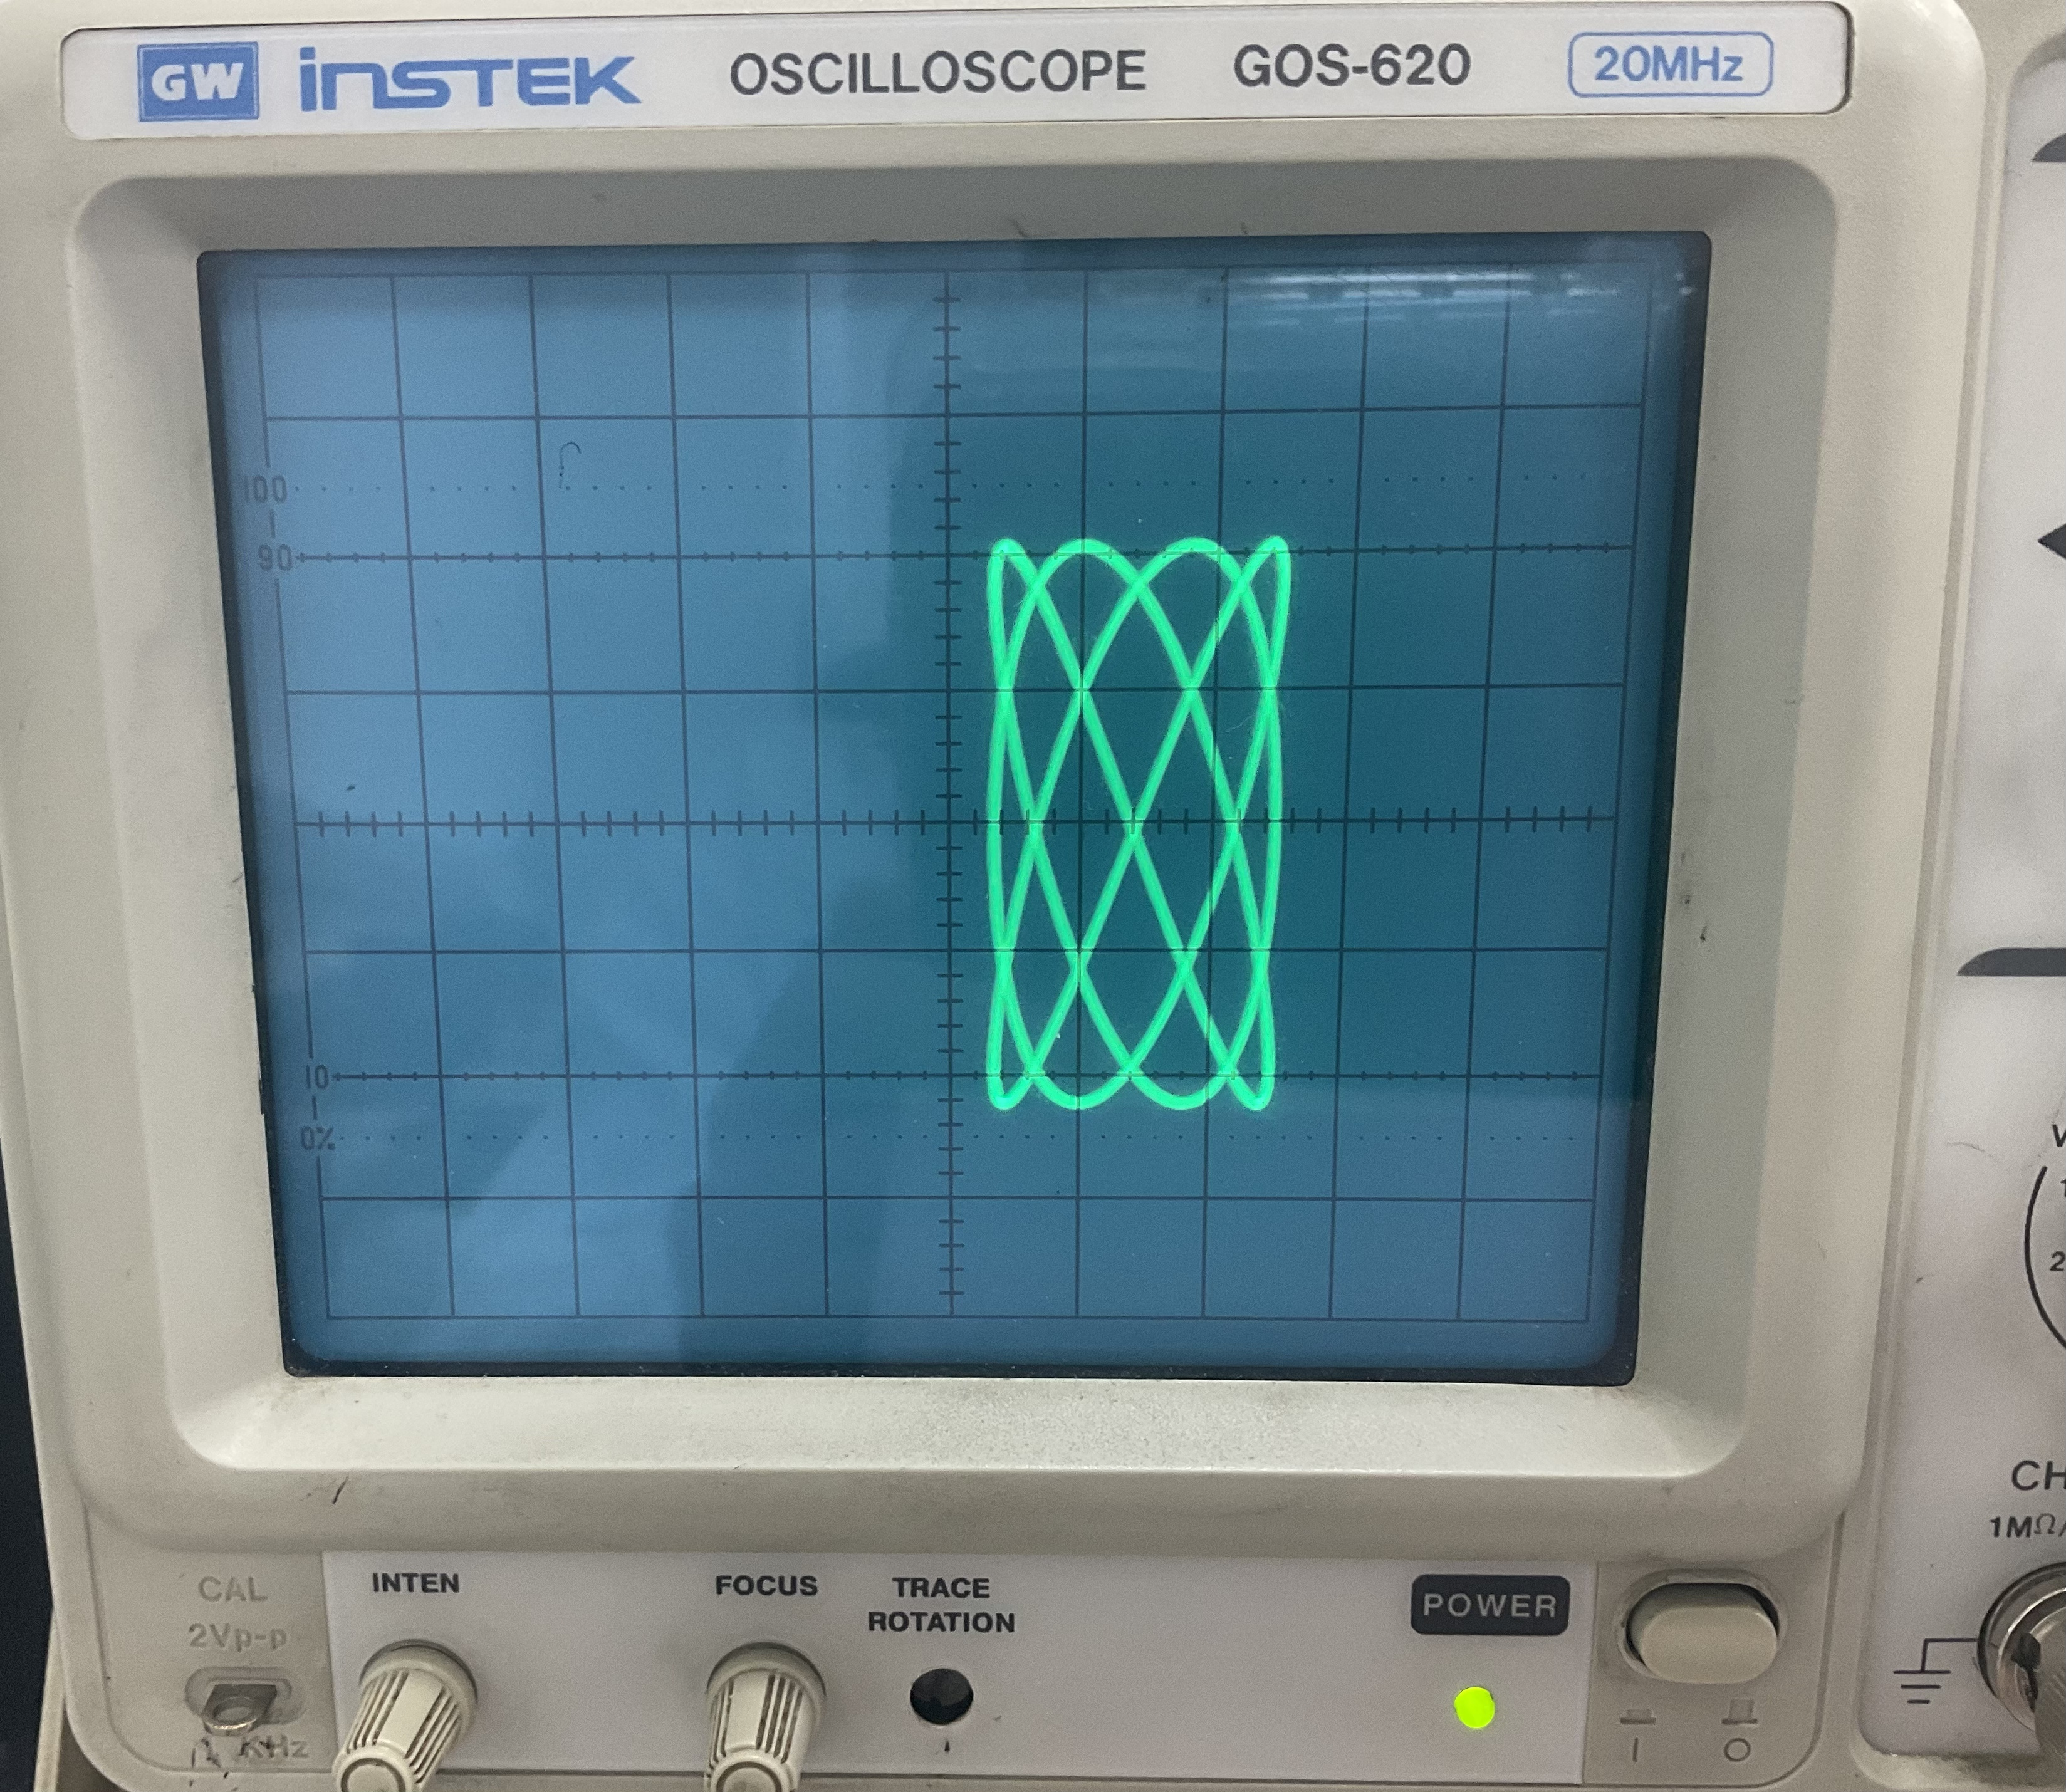
\includegraphics[width=0.9\linewidth]{img1/3比4.jpg}
		\caption*{$f_x:f_y=3:4$}
	\end{minipage}
	%\qquad
	%让图片换行,
\end{figure}

\begin{figure}[H]
    \centering
    \includegraphics[width=0.49\linewidth]{img1/3比5.jpg}
    \caption*{$f_x:f_y=3:5$}
\end{figure}


\subsection{用示波器测电压}
由原始数据可知记录得垂直衰减选择旋钮对应为$2.00 \ V$;经计算得原始数据处理后如下:

\begin{table}[H]
    \centering
    \caption{用示波器测电压}
    \begin{tabular}{|c|c|c|c|c|}
    \hline
        信号发生器电压输出值$/V$ & 2 & 5  & 7 & 10   \\
    \hline
        峰值$/V$ & $1.2$ & $2.7$ & $3.7$ & $5.5$ \\
    \hline
        有效值$/V$ & $0.85$ & $1.91$ & $2.62$ & $3.89$ \\
    \hline
    \end{tabular}
\end{table}

\section{思考题}
\subsection{开机后屏上无显示的原因以及开机后有亮点无扫描线的原因}
\begin{enumerate}
    \item 扫描方式选择了 $NORM$,垂直或水平位移旋钮不在适当位置
    \item 选择了 $X-Y$ 显示方式,$CH1$、$CH2$ 通道没有输入信号或两通道耦合方式
为 $GND$,$X$、$Y$ 偏置板上并未输入信号
\end{enumerate}
\subsection{荧光屏上仍只有一条粗扫描线的原因}
可能是轨迹聚焦旋钮未调整恰当,垂直衰减幅度太大

\subsection{荧光屏只显示较密集的竖直线的原因}
垂直衰减幅度太大或者聚焦旋钮没有调好

\subsection{荧光屏上波形移动但调节触发电平仍不起作用的原因}
CH1、CH2 通道选择错误,旋钮没有锁定

\subsection{示波器观察波形时$f_y << f_{\omega
}$屏上出现的波形类型以及相反的情况}
\begin{enumerate}
    \item 当$f_y << f_{\omega}$时,呈现出一个波形片段
    \item 当$f_y >> f_{\omega}$时,可以看到很多完整的波形
\end{enumerate}

\subsection{$Y$与$X$ 通道均输入正弦波信号但调节$f_x$和$f_y$均得不到李萨如图形的原因}
$TIME/DIV$ 旋钮未调到 $X-Y$ 模式


\subsection{示波器的$AC$输入与$DC$输入方式上的区别}
直流耦合DC是直通,交流直流一起过,信号的直流分量和交流分量都会被示波器显示出来

AC耦合则在BNC端和衰减器之间串联一个电容,会阻断信号的直流分量,只允许交流分量通过;会滤除直流成分,使得信号以平均值为零的形式显示

\subsection{区别示波器输入线的芯线和地线的方法}
芯线对壳是高阻的,并且需要连接示波器和信号发生器,故实验室示波器输入线两端都是插口;可知两端都是插口的线为芯线

地线是直通到地,而且一般是外层的屏蔽线,并且一端通常带有黑夹子。故一端带有黑夹子的线为地线







\end{document}